\documentclass[11pt,a4paper]{amsart}
\usepackage{setspace}
\doublespacing
\usepackage{amssymb,latexsym}
\usepackage{graphicx}
\theoremstyle{plain}
\newtheorem{theorem}{Theorem}
\newtheorem{corollary}{Corollary}
\newtheorem{lemma}{Lemma}
\newtheorem{axiom}{Axiom}
\newtheorem{proposition}{Proposition}
\usepackage{geometry}
\geometry{a4paper,left=2cm,right=2cm,top=1cm,bottom=1cm}
\theoremstyle{definition}
\newtheorem{definition}{Definition}
\usepackage{ulem} % various underlines
\usepackage{hyperref} % to insert URL 
\usepackage{graphicx} % to insert illustration
\usepackage[mathscr]{eucal} % to express a collection of sets
\usepackage{bm} % bold font in equation environment
\usepackage{color} % color some text
\usepackage{framed} % to add a frame 
\usepackage{tikz}
\newcommand*\circled[1]{\tikz[baseline=(char.base)]{
		\node[shape=circle,draw,inner sep=1pt] (char) {#1};}} % circled numbers
\usepackage{float}%do not auto repositioning
\usepackage[style=apa, eprint=false]{biblatex} %Imports biblatex package
\raggedright
\addbibresource{specms.bib} %Import the bibliography file

% $\uppercase\expandafter{\romannumeral1}$ Roman numeral
%	\begin{figure}[hbt]
	%{\centering \includegraphics[scale=0.78]{ring_algebra_semi}}
	%\caption{ring \& algebra \& semi-}\label{F:ring_algebra_semi}
	%\end{figure}
% \usepackage[style=apa, eprint=false]{biblatex} %Imports biblatex package
% \addbibresource{name_of_bib.bib} %Import the bibliography file

\begin{document}
\title{Math Notes}
\author{Jialiang Chen} 
\date{\today}
\maketitle
\tableofcontents

\section{Spatial Stochastic Process}
There are three approaches to embed a spatial structure in our stochastic process analysis. They are direct representations, non-parametric functions and spatial process models. The spatial process models could be simultaneous models and conditional models. They are very distinct models. 

The simultaneous models is a model for the complete pattern, so we have the endogeneous variables $y$ on the left-hand side, and the exogenous variables $X$ on the right-hand side. We want to explain the variable $y$ at all locations being explained simultaneously. The conditional models are mainly for prediction or priors for parameters in Bayesian hierarchical models. It is very common in literature that people explaining simultaneous models using the conditional language, which is not appropriate.

\subsection{Simultaneous Spatial Process Models}\hfill\par 
The variance-covariance matrix comes from the spatial random process you specify. For example, in the (Simultaneous) Spatial Autoregressive Process, we have the reduced form expression
\[	y = (I - \rho W)^{-1}u.	\]
It follows that (assuming $\mathbb{E}[y] = 0$)
\[	\begin{aligned}
	\operatorname{Var}(y) &= \mathbb{E}[yy']\\
	&= \mathbb{E}[(I - \rho W)^{-1}uu'(I-\rho W')^{-1}] \\
	&= (I - \rho W)^{-1}\mathbb{E}[uu'](I-\rho W')^{-1}.
\end{aligned}	\]
Therefore, 
\[		\operatorname{Var}(y)  = \sigma^{2} [ (I - \rho W)'(I - \rho W)]^{-1}	\]
under the assumption of homoskedasticty $\operatorname{Var}(u_{i}) = \sigma$ and independence.

\subsection{Conditional Spatial Process Models}\hfill\par 
The general idea is that we want to get the joint distribution $(y_{1}, y_{2}, \dots, y_{n})$ from the conditional distributions $y_{i} \mid y_{-i}$ by a process called \textit{factorization}, which is a product of the conditional and marginal distributions. 

This is not hard in time series. We have the Markov Property in time to simplify the factorization. In space, however, building a joint distribution from conditionals  does not necessarily work. We we specify distribution conditional on neighbors, and call these the \textit{Markov Random Field (MRF)}. The Hammersley-Clifford Theorem builds the connection between MRF and the joint distribution to make sure that our Markov Random Field defines a unique joint distribution, under certain (pretty restrictive) conditions. The reverse of this process is called the \textbf{Gibbs Sampling}. It should be noted that most of the time, the resulting joint distribution is \textit{not} a multivariate version of the conditionals, unless we are in the Gaussian world. 

\section{Specification of Spatial Dependence}
The spatial lag model and the spatial error models are the most common ways to specify the spatial dependence. There are also some other specifications. For example, the spatial Durbin model and the SLX models. However, these models should be taken with a grain of salts. 

$\bullet$ Be aware of the inverse problem. Different processes can yield the same pattern. For example, the heteroskedasticity in the variance-covariance matrix of $y$ could be the result of the `true' heteroskedasticity  in the error term $u$, or could be the result of uneven number of neighbors in the weighting matrix. It is usually hard to look back and infer what is the origin of the pattern. 

$\bullet$ There are some motivations for specifying the spatial dependence structure. However, there are also a lot of ad-hoc maneuvers. Need more theory to address these problems. The new economic geography critique by \textcite{gibbonsMostlyPointlessSpatial2012}. It is difficult to interpret causal effects.

\subsection{The Mixed Regressive-Spatial Autoregressive Model}\hfill\par 
The model is specified as 
\[	y = \rho Wy + X \beta + u, 	\]
where $Wy$ is the spatial autoregressive (spatial lag) term, $X$ is the regressive term and $\rho$ is the spatial autoregressive coefficient. We could write it as 
\[	(I-\rho W) y = X \beta + u.	\]

You could think $(I-\rho W)$ as a spatial filter, which adjusts for spatial correlation. This provides another, more practical reason for including the spatial structure than the behavior motivations. If $y_{i}$ are highly spatially correlated, there would not be enough variations for statistical analysis. We like variations, and $(I-\rho W)$ is a spatial filter that adjusts for it. (We still need to estimate $\rho$. )

The \textbf{Spatial Multiplier} is derived from the reduced form. We have 
\[	\begin{aligned}
	\mathbb{E}[y \mid \triangle X] &= (I-\rho W)^{-1}(\triangle X)\beta \\
	&= [I + \rho W + \rho^{2}W^{2} + \dots ] (\triangle X) \beta. 
\end{aligned}	\]

It is intuitive to see the multiplier effect by writing $(I-\rho W)^{-1}$ as a series. 

The total effect of a change in $X$ is $ (I-\rho W)^{-1}(\triangle X)\beta$, the direct effect is defined as $(\delta X) \beta$, and the indirect effect is defined as $[(I-\rho W)^{-1} - I](\triangle X) \beta$, or $[\rho W + \rho^{2}W^{2} + \dots ] (\triangle X) \beta$.

We could apply the spatial multiplier in policy analysis and to simulate the spatial imprint of a policy change by sollving the reduced form for a change in $X$. Read Valuing Access To Water - A Spatial Hedonic Approach Applied To Indian Cities by \textcite{anselinValuingAccessWater2008}.

The misspecification of the spatial lag model is basically a disaster. It is a omitted variable problem, which leads to biased and inconsistent results, and also larger standard deviations (so don't say I am not interested in inference, it also matters if you only want to see the overall result). 

\subsection{Spatial Error Model}
This model is not very interesting, as there is no substantive interpretation. An error is just an error. If there are spatial patterns in the error term, we extend our specification as far as we can, either by including new exogeneous variables, or by imposing structures on the error terms. 

The model is 
\[	y = X\beta + u	\]
with $u = \lambda Wu + e$.

The reduced form is 
\[	y = X\beta + (I-\lambda W)^{-1}e.	\]

Notice that there is simply no substantive multiplier effect. The only spatial effect is on the error term, which disappears on average. This model could be used for \textit{kriging} (spatial prediction).

The misspecification (consequence of ignoring SAR errors) is not that severe. The OLS remains unbiased, but it is not efficient. 

\subsection{Spatial Durbin Model}\hfill\par 
The spatial Durbin model has been widely used, but many of them are for wrong reasons (or, no reason). 
\subsubsection{The Classic Spatial Durbin Model}\hfill\par 
The point here is, the Classic Spatial Durbin Model is equivalent to the Spatial Error model. We start with rewriting a SAR model. 
\[	y  = X\beta + u 	\]
with $u = \lambda W u + e$. 
By substitution, we have 
\[	y = X\beta + (I-\lambda W)^{-1}e.	\]
Pre-multiply $(I-\lambda W)$ on both sides of the equation gives us
\[	(I-\lambda W)y = (I-\lambda W)X\beta + e.	\]

This is a spatially filtered variable regression (spatially filtered $y$ and $x$).

Now, we rewrite this equation as 
\begin{equation}\label{sdm}
	y = \lambda W y + X \beta - \lambda WX \beta + u.
\end{equation}

This is called the Classic Spatial Durbin Model. It is a non-linear model in $\lambda$ and $\beta$. Note that the coefficient on $WX$ is just the negative of the multiplication of the coefficients on $Wy$ and $X$. This gives us $k-1$ tests naturally, which is called the \textit{Common Factor Hypothesis}, and could be used to test if the SDM is an appropriate specification. (More on this later.)

Note that if we cannot reject $H_{0}: \lambda = 0$, then we are back to the standard regression model.

Note that the constant term is not \textit{separately identifiable}. The constant terms in $X$ is a column of $1$s. Note that the spatially lagged column of $1$s is not changed. The resulting constant term in this model is $(1-\lambda) \beta_{0}$. We can only identify this product, but not separately $\lambda$ and $\beta_{0}$. 

\subsubsection{The Unconstrained Spatial Durbin Model}\hfill\par 
Somehow, people started estimating
\[	y = \gamma_{1}Wy + X\gamma_{2} + WX\gamma_{3} + u,	\]
which is totally fine. But it is important to realize that the \textit{common factor hypothesis} is still there. We can test for the null hypothesis (scalar multiplication here, $\gamma_{1} \in \mathbb{R}$ and $\gamma_{2}, \gamma_{3} \in \mathbb{R}^{k}$.)
\[	\operatorname{H_{0}}:\quad \gamma_{1} \gamma_{2} = -\gamma_{3}.	\]
We are in an awkward place here. If $H_{0}$ is \textit{not} rejected, then we are in equation (\ref{sdm}), which is nothing but the SAR error model. \emph{And recall that, there is no multiplier effect in the error model.} If the $H_{0}$ is rejected, the problem is we do not know where to go - we have different interpretations. We know that this is not an SAR error process, but if we also reject $H_{0}: \gamma_{3} = 0$, this does not imply the spatial lag model. This means that these models are not nested here. 

The reduced form is 
\[	y = (I-\gamma_{1}W)^{-1}X\gamma_{2} + (I-\gamma_{1}W)^{-1}WX\gamma_{3} + v,	\]
where $x = (I-\gamma_{1}W)^{-1}u$.

Now, to look for the direct and indirect effect, we expand the inverse term out, and get
\[	y = (I + \gamma_{1}W + \gamma_{1}^{2}W^{2} + \dots )X\gamma_{2} + (I+\gamma_{1}W + \gamma_{1}^{2}W^{2} + \dots )WX\gamma_{3} + v.	\]

This is by no means simple. Note that a change in $X$ has multiple spatial effects. It is argued that the spatially lagged model already has $WX$ in it, so by adding $WX$ in addition to $Wy$, we have it twice. There should be a reason why it should be there twice. This makes the interpretation of the direct and indirect effects very complicated. 

\section{Specification of Spatial Heterogeneity}\hfill\par 
\subsection{Spatial Regimes}\hfill\par 
\subsubsection{Heterogeneity in the intercepts}
$\bullet$ Varying intercepts. The standard $t-$tests are not correct in the presence of spatial autocorrelation. In order to fix that problem, we could turn the tests (e.g., the ANOVA tests) into regression forms by adding indicator variables for each regimes, which is equivalent to the original tests, and then incorporate spatially lagged variables if necessary (as suggested by specification tests). 

$\bullet$ Spatial fixed effects. Usually in muli-level specification, for example, the units in census tracts. We include a reference mean $\alpha$ and the differences by regimes in the regression as follows
\[	y_{ij} = \alpha + \alpha_{2}d_{i2} + \dots + \alpha_{G}d_{iG} + x_{i}'\beta + \epsilon_{ij}.	\]
Note that if we include the spatial fixed effects, then we do not want to include the tract level variables as it would be superfluous. A common misconception in the literature is that spatial fixed effects "fix" the spatial autocorrelation. It only does for very specific cases. And those cases are pretty unlikely to hold. However, in some cases, after introducing the spatial fixed effects, there is no more evidence of residual spatial autocorrelation. So it has been "fixed". This is more of an empirical matter rather than a general rule. 

\subsubsection{Full Heterogeneity: Full Spatial Regimes}
This basically boils down to running a separate model in each of the subsets. The classical setup is 
\[	\begin{bmatrix}
	y_{1}\\
	y_{2}
\end{bmatrix} = \begin{bmatrix}
X_{1} & 0 \\
0 & X_{2}
\end{bmatrix} 
\begin{bmatrix}
	\beta_{1} \\
	\beta_{2}
\end{bmatrix} + 
\begin{bmatrix}
	\epsilon_{1}\\
	\epsilon_{2}
\end{bmatrix}.	\]
If there are no correlations across regimes, then it is better to write two regression equations instead.

\subsection{Testing for Spatial Heterogeneity}
 Our null hypothesis is equal intercepts and equal slopes.  The classical test on structural stability in econometrics is the Chow test \footnote{The Chow test is named after the Chinese-American economist Zhizhuang Zou.}. The basic idea is comparing two models - the restricted model and the unrestricted model. "Restricted" means you restrict some coefficients to be zero, and the "unrestricted" can be any number. Therefore, the restricted is always the simpler model. In our context, the "restricted" means all the coefficients are the same everywhere, and the "unrestricted" means flexibility for each of the subsets. 
 
 We could generalize the Chow test for a general test on coefficient variability. As an example, suppose we run two separate regressions for the regimes and get a full vector for the estimands $\beta' = (\beta_{11} \beta_{12} \beta_{13} \beta_{21} \beta_{22} \beta_{23})'$. We supply a matrix $R$, for example, specified as 
 \[	R  = \begin{bmatrix}
 	1 & 0 & 0 & -1 & 0 & 0 \\
 	0 & 1 & 0 & 0 & -1 & 0 \\
 	0 & 0 & 1 & 0 &  0 & -1
 \end{bmatrix}.	\]
Then our null hypothesis would be 
\[	H_{0}: R\beta = 0.	\]

This is a chi-square statistic ( a generalized Wald test), following the distribution 
\[	(R\hat{\beta})'[RVR']^{-1}(R\hat{\beta}) \sim \chi^{2}(G),	\]
where $V$ is the variance-covariance matrix of the $\hat{\beta}$. The tricky part lies on the identification of $V$. 

Note that this is perfectly flexible. You can test if $\beta_{12} = 2 \beta_{22}$ easily for example. Also, as long as you can come up with the $V$, no matter it comes from the spatial autoregressive model or the spatial lag error model.

\subsection{Spatial Regimes with Spatial Dependence}
We know how to deal with the regression coefficients part, but how should we deal with the spatial part? Do we keep the spatial process the same throughout? There is no clear direction except for simplicity. 

The spatial econometrics is based on asymptotics, and we need to think about the issue of whether the limit process stops at the border between regimes. Do not change the process unless you have a strong foundation. 

We have the two-regime spatial lag model with fixed spatial autoregressive coefficient
\[	\begin{bmatrix}
	y_{1}\\
	y_{2}
\end{bmatrix} = \rho W
\begin{bmatrix}
	y_{1}\\
	y_{2}
\end{bmatrix} + 
\begin{bmatrix}
	X_{1} & 0 \\
	0 & X_{2}
\end{bmatrix} 
\begin{bmatrix}
	\beta_{1}\\
	\beta_{2}
\end{bmatrix} + 
\begin{bmatrix}
	\epsilon_{1}\\
	\epsilon_{2}
\end{bmatrix}.	\]

The two-regime spatial lag model with varying spatial autoregressive coefficient is 
\[	\begin{bmatrix}
	y_{1}\\
	y_{2}
\end{bmatrix} = 
\begin{bmatrix}
	\rho_{1}W_{1} & 0 \\
	0 & \rho_{2}W_{2}
\end{bmatrix}
\begin{bmatrix}
	y_{1}\\
	y_{2}
\end{bmatrix} + 
\begin{bmatrix}
	X_{1} & 0 \\
	0 & X_{2}
\end{bmatrix} 
\begin{bmatrix}
	\beta_{1}\\
	\beta_{2}
\end{bmatrix} + 
\begin{bmatrix}
	\epsilon_{1}\\
	\epsilon_{2}
\end{bmatrix}.	\]
Note that there is no spillover between the two regimes. Similarly for the spatial error model.

\subsection{Spatially Varying Coefficients}\hfill\par 
\subsubsection{Expansion Method}
One way to deal with varying coefficients is by imposing structures on the coefficients. The initial model would be 
\[	y_{i} = \alpha + x_{i}\beta_{i} + \epsilon_{i}.	\]
Note the extreme heterogeneity here. This is an incidental parameter problem. We have the expansion equation
\[	\beta_{i} = \gamma_{0} + z_{i1}\gamma_{1} + z_{i2}\gamma_{2}.	\]
Some algebra shows that 
\[	y_{i} = \alpha + x_{i}\gamma_{0} + (z_{i1}x_{i})\gamma_{1} + (z_{i2}x_{i})\gamma_{2} + \epsilon_{i}.	\]
We ended up with a equation with interaction effects. We should be aware of the multicollinearity problem and the danger of overfitting. We can also let random error presents in the expansion equation
\[\beta_{i} = \gamma_{0} + z_{i1}\gamma_{1} + z_{i2}\gamma_{2} + \psi_{i}\]
and get the random expansion model.

\subsubsection{Geographically Weighted Regression}\hfill\par 
This is a special case of local regression. Local regression is about the attribute spaces, the space of variables $y$ and $x$s.  GWS is about the geographical space. Classical local regression exploits local subsets in the attribute dimensions, GWS exploits local subsets of the attribute, but in geographic space. The parameter values are obtained from a subset of observations using kernel regression. 

Suppose we are interested in the conditional expectation, i.e., the regression. For a simple bivariate regression, we have 
\[	y_{i} = m(x_{i}) + u_{i},	\]
where $m$ is an unspecified functional form. The kernel regression would be 
\[	m(x_{0}) = \sum_{i} K[(x_{i} - x_{0})/h] y_{i},	\]
where $K$ is our kernel function, and $h$ is the bandwidth. This is the classic kernel regression.

In the GWR setup, local estimation is based on nearby locations. But note that our local estimation is now based on the $x-y$ pairs at nearby locations. This give us a difficulty for interpretation - there is simply no asymptotics by adding more units in the nearby locations. Mathematically, we have 
\[	b(u_{i}, v_{i}) = [X'W(u_{i}, v_{i})X]^{-1}X'W(u_{i}, v_{i})y,	\]
where $W(u_{i}, v_{i})$ is a matrix with weights in the diagonal elements.

To carry out with GWR, we should be aware of the choice of bandwidth, parameter inference and the visualization.

\subsection{Spatial Random Effect}\hfill\par 

\section{Maximum Likelihood Estimation}
\subsection{Spatial Stationarity}\hfill\par 
 It is important to realize that the spatial pattern is just a realization of the spatial stochastic process, rather than multiple realizations in the map. Of course we are in trouble because you cannot infer the whole process from just one realization. The challenge here is how to treat map as if it has multiple data points (as different realizations of a random variable). In order to do this, we need to make strong assumptions pertaining a notion of equilibrium. The whole notion of \textit{stationarity} is a notion of equilibrium of the stochastic process such that we can do this. (Note that we are still in the cross-sectional world). 
 
Our stationarity condition is 
\[	\{z(s_{1}), \dots, z_{s{k}}\} \quad \text{and}\quad \{z(s_{1+h}), \dots, z({s_{k+h}})\} \quad \text{have the same distribution for all $k$ and all $h$}.	\]

This is pretty unrealistic. A weaker condition would be the moment stationarity. This pertains to certain moments of the joint distributions. Keep these burdens on the model in mind. 

\subsection{Ergodicity}
 No matter which map we are looking at, we are getting the same information in terms of the process. 

\subsection{Asymptotics in Space}\hfill\par 
Uniform Law of Large Numbers
\[	(1/N)\sum_{i}[g_{i}(x, \theta) - Eg_{i}(x, \theta)] \rightarrow 0.	\]
$g$ is a function of data, could be the maximum of the likelihood function, or the minimum of the sum of squares, or other objective function.

Central Limit Theorem: It's actually about how you go to the limit. In the limit, there is no uncertainty. The man deviation of a function computed for the "sample" from its expressed value converges to zero.  

In space, we can go to the limit in different ways, and it matters. 
\subsubsection{The Increasing Domain Asymptotics (Kansas Model)}\hfill\par 
Unbounded space, infinite range, expands at the edges. Create boundary effect. The number of neighbors does not depend on $N$.
\subsubsection{The Infill Asymptotics (Sandbox Model)}\hfill\par 
Here the space is bounded. We ge to the asymptotic world by adding additional observations in the sandbox. Here the number of neighbors increases in $n$. 

\subsection{ML Estimation Principle}\hfill\par 
In ML Estimation, you maximize the likelihood, and the likelihood is the  joint probability of the sample. In order to figure out what the joint probability of the sample might be, we need a probability density function. ML is highly parameterized, and we need to make a lot of assumptions. It contracts with the methods of moments. 

We think of the data as a sample from a fully specified distribution with a set of (pre-determined) parameters. Then we move to find the parameters that \textit{maximizes} the joint probability of the sample.

The likelihood function is the expression of the joint probability of the sample as a function of data and parameters
\[	L(\theta \mid X) = f(x_{1}, \dots, x_{n}, \theta).	\]

Note that this is a likelihood function in the classical context, instead of in the Bayesian context. In the  classical context, the likelihood is a function that determines the parameters, conditional on the data. In Bayesian world, it is the other way around since all the parameters have a distribution (they are constants in the classical world).  

For independent observations, this is the product of the individual observations. And if we take the log form, we have the \textit{log-likelihood function} as a sum.
\[	\ln L(\theta \mid X) = \sum_{i} \ln f(x_{i}, \theta).	\]

But this is no longer the case in spatial econometrics, as they are not independent. We have to deal with the joint probability as a whole. This is a fundamental difference. 

We have to solve the optimization problem. We take the first order derivatives of $\ln L$ with respect to $\theta$ to solve for the parameter values. There is often no analytical solutions, so numerical optimization is necessary. 

This is a point estimate, now we want to say something about the variability of the estimate. This is where the asymptotics kicks in.
 
\textit{The Fisher Information Matrix} is defined as the negative expected value of the second order partial derivatives of the log-likelihood function. And the inverse of the information matrix is the asymptotic variance.  

MLE is highly parametric: it has lots of informations, but if assumptions hold, it is optimal. It is consistent and asymptotic efficient  (the smallest asymptotic variance among consistent estimators). It is also asymptotically normal.

$\bullet$ \textit{The invariance property} Note that the expected value of a function is not necessarily a function of the expected value.  But we are in the asymptotic world and dealing with these maximum likelihood estimates, anything goes. This is useful for policy analysis - our estimates can be used in calculations in the place of the true (unknown) parameter values.

In spatial econometrics, because of the dependency of data, things are very complicated. This requires specialized laws of large numbers and central limit theorem. See the next section.

\subsection{ML Estimator of Spatial Lag Model}\hfill\par 
The main issue with the spatial lag model is the endogeneity. Specifically, the spatially lagged $y$ is directly correlated with the error term. The only way we can do this is to have a formal model for the randomness in this process. Remember that our model is 
\[	y = \rho Wy + X\beta + e.	\]
Note that the randomness is in the error term. So the randomness in $y$ is only because of the randomness in the error term. Therefore, we make assumptions about the parametric model for the randomness in the error term. Typically, we assume a multivariate normal distribution (multivariate because these things are dependent, so we have to work with the whole thing in one shot). So $e \sim \mathscr{N}(0, \sigma^{2}I)$. We get the randomness for the $y$ as a transformation from the randomness in the error terms. 

The log-likelihood for joint density $e \sim \mathscr{N}(0, \Sigma)$ takes the form
\begin{equation}\label{log-likelihood}
	\ln L = -(n/2) \ln(2\pi) - (1/2) \ln |\Sigma| - (1/2) e'\Sigma^{-1}e.
\end{equation}
Note that the last term is a sum of squares, so $\max \ln L$ is equivalent to minimizing the weighted least squares as the other terms are constants. An immediate problem is that we do not observe them. But we do have a functional relationship between $e$ and the observed variable $y$ as 
\[	e = (I - \rho W)y + X \beta \quad \text{or} \quad e = f(y).	\]

Now, the likelihood of $y$ follows from the variable transformation, which requires Jacobian of the transformation.  The Jacobian of a transformation rescales the distribution so that the distribution of the transformed variable is proper. Formally, it is the determinant of an $n-$by$-n$ matrix
\[	\det (\partial f/\partial y) = \det (I - \rho W).	\]
This is a long way of saying that we need to change the likelihood function. Note how this not a problem in the standard regression: we have $\partial f/\partial y = 1$. 

Now, the  log-likelihood for joint density is 
\[	\ln L = -(n/2) \ln(2\pi) -(n/2)\ln \sigma^{2} + \ln |I-\rho W| - (y - \rho Wy - X \beta)'(y - \rho Wy - X \beta)/(2\sigma^{2}).	\]

(Recall that we assumed $e \sim \mathscr{N}(0, \sigma^{2}I)$) 

Note that the Jacobian of the $n-$by$-n$ matrix $I-\rho W$ enters the function directly. We can use numerical optimization to find the parameter values that yield $\max \ln L$, but it can be computationally intensive.

The good news is that there are actually analytical solutions for $\beta$ and $\sigma^{2}$ from the FOCs. But we still need to get $\rho$. We then take the expressions for  $\beta$ and $\sigma^{2}$ and substitute them back to the likelihood function to get a \textit{concentrated likelihood function}. The resulting function is 
\[	L = -(n/2) \ln [(e_{0}-\rho e_{L})'(e_{0}-\rho e_{L})/n] + \ln |I-\rho W|.	\]

This is a nonlinear optimization problem over a single parameter. The parameter space turns out to be $(1/\omega_{\min}, 1/\omega_{\max})$ , where the endpoints are the minimal and maximal eigenvalues of the weights matrix. 

Our information matrix is 
\[	I(\theta) = - \mathbb{E}[\partial^{2} \ln  L/\partial \theta \partial \theta'],	\]
and the asymptotic variance is just the inverse of it (and there is no analytical expression). The usual simplifications do not work, and partial derivatives explicitly needed for the information matrix. 

The important thing to notice that the precision of the parameters of the error term ($\sigma$ is one of them) affects the precision of the $\rho$. This is a fundamental difference between pretty much anything in standard econometrics. This is peculiar in the spatial econometrics. 

Then the asymptotic variance matrix is just the inverse of the information matrix, but there is no analytical expression. But it is not block-diagonal between $\rho$ and $\sigma^{2}$. For a feasible generalized least square estimator, we only need a consistent estimator of the error parameter and it does not need to be efficient because the efficiency does not matter (it is block-diagonal). We will come back to t his when we talk about methods of moments later on. 

\subsubsection{Predicted Values and Residuals}\hfill\par 
The predicted value from structural form is not valid. We need to use the reduced form 
\[	\mathbb{E}[y \mid X] = (I - \rho W)^{-1}X \beta = (I + \rho W + \rho^{2}W^{2} + \dots) X \beta.	\]

As for the residuals, the naive residual would be 
\[	u = y - \rho W y - X \beta = (I - \rho W)y - X \beta.	\]
This is fine, and it is actually the one being used in the specification tests.

The other way to get residuals is to use the reduced form, which gives
\[	u = y - (I - \rho W)^{-1}X\beta.	\]

\subsection{Maximum Likelihood Estimation of the Error Models}

We use the Spatial Autoregressive Error model for illustration and for simplicity. We have 
\[	e = \lambda We + u.	\]

The non-spherical variance matrix for the error term is 
\[	\Sigma = \sigma^{2}[(I-\lambda W)'(I - \lambda W)]^{-1}.	\]

The SAR error model is simpler since there is an inverse in the $\Sigma$. Therefore, the inverse variance-covariance matrix $\Sigma^{-1}$ (used in the Generalized Least Squares) does not contain inverse terms anymore.

$\lambda$ here is a nuisance parameter, which means that it is not of the direct interest of itself, but important in estimation of $\beta$. This is actually the problem of efficiency as our $\beta$ remains unbiased under misspecification as we haven seen before. 

$\bullet$ Generalized least squares methods, aka Spatially Weighted Least Squares here.
We have the Generalized Least Squares Estimator
\[ b_{GLS} = [X'\Sigma^{-1}X]^{-1} X'\Sigma^{-1}y. \]

By substituting $\Sigma^{-1} = 1/\sigma (I-\lambda W)'(I - \lambda W)$, we get the Spatially Weighted Least Squares estimator
\[	b_{SWLS} = [X'  (I-\lambda W)'(I - \lambda W) X]^{-1} X'  (I-\lambda W)'(I - \lambda W) y = [X_{L}'X_{L}]^{-1}X_{L}^{'}y_{L},	\]
where $X_{L} := (I-\lambda W)X$ and $y_{L} := (I-\lambda W)y$ are spatially filtered  variables. 

The last expression should be familiar to you. If we knew $\lambda$, then we are back to OLS.

Now, the main business is to get $\lambda$. Unfortunately, we have to go through the whole process of the MLE. We assume the normality of error terms, and that yields the normality of the dependent variable, then we spell out the likelihood function, and do the optimization problem to get a consistent estimate for $\lambda$. There is no shortcut. 

The log-likelihood function is 
\[	\ln L = -(n/2)\ln(2\pi) - (n/2) \ln \sigma^{2} + \ln |I -\lambda W| - e_{L}e_{L}^{'}/(2\sigma^{2}),	\]
where $e_{L} = (I-\lambda W) (y - X\beta)$, and $ |I -\lambda W| $ is our Jacobian.

We also need to resort to numerical optimization to find parameter values that yield $\max \ln L$.

We can also turn the optimization problem to a single parameter optimization problem as we did before. 

Some software do not bother with the variance of $\lambda$, as it is complicated (mostly due to the inverse). But there are ways for inference to get around of this. (More on this later.)

It should be noted that the asymptotic variance matrix is black diagonal in this case. There is no correlation between the ($\lambda$  $\sigma^{2}$) and $\beta$. For feasible generalized least squares, all we need is a consistent estimate for the nuisance parameter.  At the end of the day, the precision of $\lambda$ does not affect that of $\beta$.

\subsubsection{Predicted Values and Residuals}\hfill\par 
There is no effect of error variance on point estimates, but the effect is on precisiion of estimate. 

The residuals are a little confusing, the unfiltered is $u = y - X \beta$, and you will find that there are some spatial correlation. They are indeed. The filtered one $u = (I-\lambda W) y - (I -\lambda W) X\beta$. 

\subsection{Model Comparison}\hfill\par 
$\bullet$ $R^{2}$ is no longer an appropriate measure of fit as it is based on unweighted sum of squared residuals. Use the Pseudo $R^{2}$. It is based on the squared correlation between observed and predicted values, and does not have the classic interpretation of "explained variance/total variance". Usually larger is better.

$\bullet$ Maximized Log-Likelihood This is not a measure of fit, but a measure of relative model adequacy of tthe same dependent variable. In general, highest value (least negative) is best.

$\bullet$ Some notion for the adjusted $R$-square: \textit{information criteria}. e.g., Akaike Information Criterion. Smallest AIC is the best. Only the relative comparison is meaningful. 

\subsection{Computational Issues}\hfill\par 
The log-likelihood functions in spatial econometrics are not standard. We have to model the joint distribution. Everything is about multivariate normal. To apply maximum likelihood for a count variable using Poisson distribution, the joint distribution and marginals are complicated (they are usually not of the same type). That is part of the reason why the approach taken in the literature is an indirect approach in a hierarchical specification  with a random effects specification. We do not model the counts directly, but model the intensity parameters. So it is a randomly varying parameter that has a component that is spatially dependent. 

The presence of the Jacobian term is another source of complexity. It is a computation beast. There are also other large matrix expressions that are complicated. You can do sometime like writing the determinant as a product of the eigenvalues. But eigenvalues are not easy to compute.  

We cannot have endogenous variables (therefore no IV) in the maximum likelihood estimation, and we need to have our weights are intrinsically symmetric. 

The preferred approach is not to use maximum likelihood, for two big reasons:
\begin{enumerate}
	\item It is very difficult to maintain that all the variables on the right-hand side variables are exogenous. But ML assumes them away.
	\item Heteroskedasticity. It is normal. But ML here basically ignores that.
\end{enumerate}

Remember the assumptions you make in the maximum likelihood: Normal distribution, variance constant. If these assumptions are violated, then we need to take that into account in the likelihood function. If we do not do that, we are still maximizing a likelihood function, but it could be the wrong one. And this can be serious in the sense that you lose your consistency in some circumstances.

\section{Specification Tests}\hfill\par 
Some of the standard regression assumptions may be violated in practice, for example, the OLS $2$ assumption. We want to detect if this is the case. The motto of specification testing is to establish the formal connection between something that we compute for the \textit{residuals} (i.e., the difference between the predicted values and the true values) and something that is relevant for the unobservable error terms. 

The classic linear regression is 
\[	y = X \beta + e,	\]
where $\mathbb{E}[ee'] = \sigma^{2}I$. (So uncorrelated error terms and homoskedasticity.)

The important assumptions here are
\begin{enumerate}
	\item Correct specification. The true data generating process is actually linear.
	\item Error terms. Test for covariance and heteroskedasticity. The error term could be spatially autocorrlated. (e.g., a SAR process).  Recall our inverse problem: the unbalanced neighbors will produce heteroskedasticity even if there is no heteroskedasticity in $e$. Is there any approach to separately detect that?
	\item  Exogeneity $\mathbb{E}[e'X] = 0$. If there is endogeneity, it is usually hard to address in maximum likelihood setting. We prefer general methods of moments.
\end{enumerate}

Usually, specification test for one type typically have power for multiple types of misspecification. This complicates things. 

If our test tells us that we need incorporate spatial structure into our OLS model, we will turn our attention to the spatial lag model or SAR error model. The later two are our "unconstrained" models (our alternative hypotheses), and by setting respective parameters to $0$, we will come back to the "constrained" model, the OLS. 

\subsection{Types of Tests}\hfill\par 
The formal structure of of hypothesis is 
\[	H_{0}: \text{constrained model} \qquad H_{1}: \text{unconstrained model}.	\]

For spatial lag model, we have 
\[	H_{0}: \rho = 0 \qquad H_{1}: \rho \ne 0.	\]

For spatial error model, we have 
\[	H_{0}: \lambda = 0 \qquad H_{1}: \lambda \ne 0.	\]

There are two board types of tests.

$\bullet$ \textit{The Diffuse Tests.} This means the tests that have no specific alternative. For example, 
\[	H_{0}: \text{no spatial autocorrelation} \qquad H_{1}: \text{there actually is}.	\]
Basically, we want  to make sure that our specification is correct. If we reject $H_{0}$ in favor of $H_{1}$, the only thing we know is that there exists spatial autocorrelation. It could be the autoregressive model, moving average, the lag or the error models. These are like different favors of Moran's I. 

$\bullet$ \textit{The Focused Tests.} This means the tests that have specific alternative. For example, 
\[	H_{0}: \text{$\rho = 0$ in a spatial lag model.} \qquad H_{1}: \text{$\rho \ne 0$ in a spatial lag model.}	\]
This is a significance test on $\rho$. Most of these focused tests are in highly parametric maximum likelihood frameworks. The examples include Wald test (asymptotic t-test), Likelihood Ratio test (LR), and Lagrange Multiplier test (LM), 

Note that since we need a fully specified model, we need to make assumptions, and these assumptions may not hold. That means we may need specification tests for specification tests and so on. In classical statistics, the $p-$value of a test is valid only if that test is carried out in isolation. If one test is carried out after another test, we call this \textit{pre-testing}. In these scenarios, the $p-$value of the second test depends on what you decide (which is a statistical decision, and could be wrong!) in the first step. This is the same problem in the multiple test, and the $p-$values are not reliable. If you test long enough, it is going to be significant anyway. 

In practice, people have instantaneous amnesia. Read more about the misuse of p-values. If you are way under the cutoff, you are fine. But if you are near the boundary, be very wary. The $p-$values are not reliable.

\subsection{Diffuse Test: Moran's I}\hfill\par 
We work with the residuals as we do not observe errors. The Moran's I statistics is defined as 
\[	I = \frac{u'Wu/S_{0}}{u'u/N}, \qquad \text{with} S_{0} = \sum_{ij} w_{ij}.	\]
Note that the numerator is a sum of the cross produce between the residual and its spatial lag, divided by the sum of all weights. The denominator is just the variance. For row-standardized weights, $S_{0} = N$ and hence $I = u'Wu/u'u$.

The inference is not straightforward, but based on a asymptotic normal approximation. First we build the connection between the residual and the error terms
\[	\begin{aligned}
	u &= y - X[(X'X)^{-1}X'y] \\
	&= [I - X(X'X)^{-1}X'](X\beta + e)\\
	&= (X\beta - X\beta) + [I - X(X'X)^{-1}X']e\\
	&= Me,
 \end{aligned}	\]
where $M := [I - X(X'X)^{-1}X'$ is an \textit{idempotent matrix}\footnote{This is everywhere in advanced econometrics} with the properties 
\[MM = M = M' = M'M. \]

Note that we write $u$ as a linear transformation of the true error terms $u$. However, $M$ is not invertible. Actually we can get $n-k$ uncorrelated residuals from this, which is the degree of freedom. This imperfect connection is good enough for us. 

Given the null assumption about $e$ (not spatially correlated), we can figure out the properties of $u$ through this equation. We need to derive asymptotic normality of $I$. As a first step, we compute the expectation of $I$.

We have 
\[	\mathbb{E}[u'u]  \stackrel{(1)}{=} \mathbb{E}[e'Me] \stackrel{(2)}{=} \mathbb{E}[tr(e'Me)]  \stackrel{(3)}{=} \mathbb{E}[tr(Mee')]  \stackrel{(4)}{=} \sigma^{2}tr(M)  = \sigma^{2}(N-k).	\]
(1) is by substitution, (2) is because $e'Me$ is a $1-$by$-1$ matrix, (3) is by the property of trace of a matrix, (4) is by our assumption that $\mathbb{E}[ee'] = \sigma^{2}I$.

Similarly, we have 
\[	\mathbb{E}[u'Wu] = \sigma^{2} tr(WM). 	\]

It follows that 
\[	\mathbb{E}[I] = tr(MW) / (N-K)	\]
and 
\[ \operatorname{Var}(I) = (T / [(N-K)(N-K-2)]) - (\mathbb{E}[I])^{2},	\]
where $T$ is a complicated number.

After proving a asymptotic normality property, we can use the standardized z-value 
\[	z(I) = \frac{I-\mathbb{E}[I]}{\sqrt{\operatorname{Var}(I)}}	\]
 for testing.
 
 Note that permutation is never an option for Moran's I derived from residuals. 
 
 You can generalize the Moran's I test statistics to other residuals. For example, the residuals in the two stage least square regressions, and residuals in a discrete dependent model. You can plug in Moran's I in the generalized residuals and do a test.
 
 Moran's I can be computationally intensive as it involves traces of big matrices, an alternative would be the Lagrange multiplier statistics.
 
 The lack of rejection means the model is correctly specified. However, the rejection for the null for Moran's I needs to be interpreted with caution: it is not clear what the alternative is. For example, it could be the error \textit{or} the lag (or both), and they can be combined with other misspecification. It is not clear which form of spatial autocorrelation might exit there.
 
 Moran's I has power against many alternatives, such as non-normality, heteroskedasticity, autocorrelation and so on. It is a great misspecification test, and not that useful in a specification search - it is not clear what the next step should be.  
 
\subsection{Classic ML-based Tests}\hfill\par 
Three are three ways of thinking about specification test in a maximum likelihood framework. 
\begin{enumerate}
	\item \textit{value} of the estimate compared to null hypothesis. This is the usual Wald test (asymptotic t-test) that we do forever, and we need standard error. 
	\item  \textit{fit of measure.} This compares the maximized log-likelihood with the log-likelihood of the constrained model. For example, the likelihood ratio (LR) test. Note that the log-likelihood is a function of our data, and therefore is a random variable also. To tell if the difference is large enough, we also need the standard error.
	\item \textit{slope} of likelihood functions compare to zero. By the first order conditions, the slope of the log-likelihood function is $0$ at the optimum. And it is not necessarily $0$ at other places. We want to tell whether that difference in slope is large enough. Note that slope is also a random variable, and we need its standard error. Example includes the Lagrange multiplier (LR) test or Rao Score test.
\end{enumerate}

They are asymptotically equivalent, and in finite samples we have $W \geq LR \geq LM$. This only holds in perfect circumstances.

\subsubsection{Wald Test}\hfill\par 
This requires the estimation of the alternative model, i.e., a spatial lag or a spatial error model. Then we use the variance estimate, and we have 
\[	t = \frac{\hat{\theta}}{\sqrt{\operatorname{Var}(\hat{\theta})}} \stackrel{d}{\longrightarrow} \mathscr{N}(0, 1) \quad \text{or}\quad t^{2} \sim \chi^{2}(1).	\]

\subsubsection{Likelihood Ratio Test}\hfill\par 
For the likelihood ratio test, we actually need to estimate two models: the unconstrained (spatial) and the constrained (non-spatial). The test statistics follows a $\chi^{2}$ distribution with degree of freedom $1$. 
\[	LR = 2[L(\theta) - L(\theta = 0)] \sim \chi^{2}(1).	\]
Note that the unconstrained one always have a larger (in a non-strict sense) likelihood (or, "better fit") than the constrained. If not, something must be wrong and check your calculation.
 
 Probably more powerful. Use more info.
  
\subsubsection{Lagrange Multiplier Test}\hfill\par 
 The advantage of LM test is that we only need the estimation of the null model. But the derivation is quite painful.

$\bullet$ \textbf{LM Error Test/ Score Test}
\[	LM_{\lambda} = \frac{d_{\lambda}^{2}}{T} \sim \chi^{2}(1) \qquad \text{with} \quad d_{\lambda} = \frac{e'We}{\hat{\sigma}^{2}_{ML}},	\]
where $T = tr(WW + W'W)$.

Moran's  I and the LM Error Test are vary similar. 

$\bullet$ \textbf{LM Lag Test} 
\[	LM_{\rho} = \frac{d^{2}_{\rho}}{D} \sim \chi^{2}(1) \qquad  \text{with} \quad d_{p} = \frac{e'Wy}{\hat{\sigma}^{2}_{ML}},	\]
where $D = (WX\hat{\beta})'[I - X(X'X)^{-1}X'](WX\hat{\beta}) / \hat{\sigma}^{2}_{ML} + T$. 

One problem with these LM test is that the lag test has power against the error model, and vice versa. If one of the other alternative is present, then the distribution becomes a non-central chi square distribution, and the robust version shifts it back to the central chi square distribution.

$\bullet$ \textbf{The Robust LM-Error} 
We have
\[	LM_{\lambda}^{*} = \frac{(d_{\lambda} - TD^{-1}d_{\rho})^{2}}{T(1-TD)} \sim \chi^{2}(1).	\]


$\bullet$ \textbf{The Robust LM-Lag}
We have 
\[	LM_{\rho}^{*} = \frac{(d_{\rho} - d_{\lambda})^{2}}{((D-T))} \sim \chi^{2}(1).	\]

Note that we should only use the robust tests when both LM-Error and LM-Lag reject the null, and do not use the robust tests when neither of the LM-Error and LM-Lag are significant. 

\subsection{Higher Order Tests}\hfill\par 
The test on SARMA has the null hypothesis $H_{0}: \lambda = \rho = 0$, and the test statistic is 
\[	LM_{\rho \lambda} = \frac{d_{\lambda}^{2}}{T} + \frac{(d_{\lambda} - d_{\rho})^{2}}{D-T} \sim \chi^{2}(2).	\]

We should be cautious with the interpretation of the SARMA test. A significant result does not necessarily mean that the altervative is a higher order model. Note that the test statistic is a sum of two - the LM Error + Robust LM-Lag (or LM - Lag +  Robust LM - Error). So if one of them is exceedingly high, the overall result is also significant. Do not rush to higher order models, but go to weight matrix etc. Simple models are always better.

\subsection{Generalized Moran's I test}

We can extend the Moran's I tests to residuals other than OLS, for example, the 2SLS regression.

\subsection{Specification Search}

The principle is how do you figure out what is a better model. Remember there is pre-testing problem. Economists and statistician care about specification test (machine learning world does not). There are two main strategies.
\begin{enumerate}
	\item forward step-wide strategy
	\item  backward step-wide strategy. The most complex model in the spatial context is actually really hard to estimate, and sometimes even impossible to estimate. 
\end{enumerate}

$\bullet$ Forward Step-Wise Strategy

We start from the constrained model, which is non-spatial, and use LM test statistics to guide model selection. We could add spatial heterogeneity or spatial dependence, and do the tests again, until the assumptions are satisfied. The problem here is pre-testing. This is awkward and there is no great solution to there theoretically. Practically speaking, this is fine.

$\bullet$ Backward Step-Wise Strategy

We start from the most complicated model we can think of, and then we move backward and test the constrains. The problem here is that this requires estimation of complex spatial models first to test parameter constrains (using Wald or LR tests). 

\begin{figure}[hbt]
{\centering 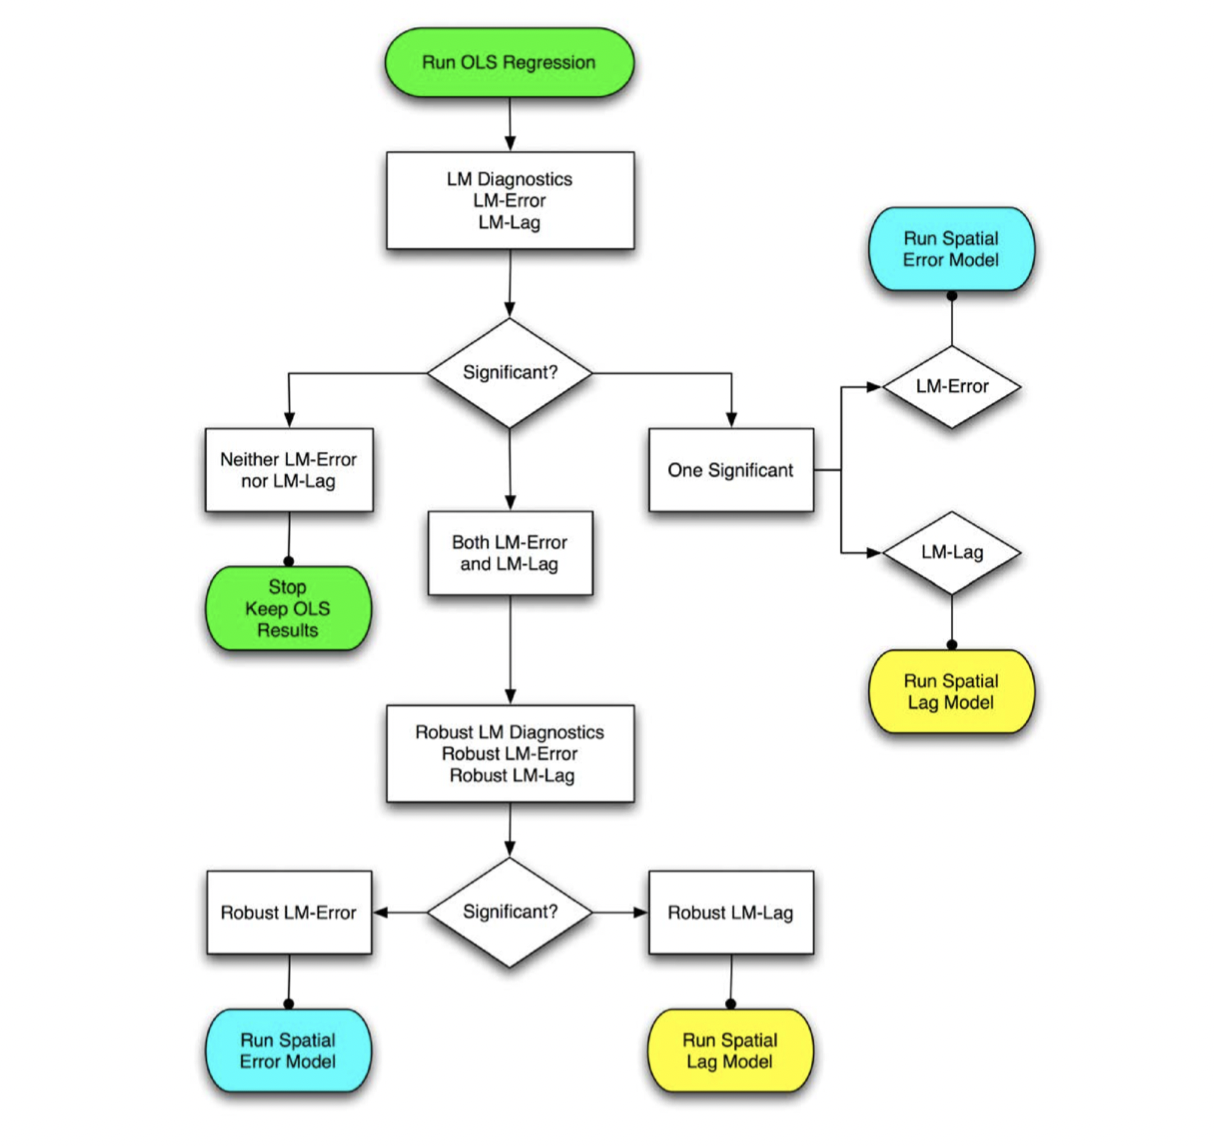
\includegraphics[scale=0.48]{flowchart}}
\caption{Flowchart for model specification}\label{F:flowchart}
\end{figure}

If both Robust tests rejects the null, and we cannot tell, then possibility of higher order model or alternative specifications. You are basically in trouble here. In this case, the specification test ceases, and we may need to go model comparisons in terms of the goodness of fit, meaning of interpretation and so on. As a rule of thumb, an error model is preferred than a lag model for economists. The lag thing is a beast. It is also frequently mis-interpretated. The price of my house does not depend on my neighbors. It is that the pattern of the prices as a whole is determined by the pattern of the explanatory variables at the location as well as the neighboring locations. 

\newpage
\printbibliography %Prints bibliography
		
\end{document}
